\documentclass[conference]{IEEEtran}
\hyphenation{op-tical net-works semi-conduc-tor}

\usepackage{graphicx}

\begin{document}
\title{Freedom Fridays: Designing 100 Faulty Lightbulbs}

\author{
\IEEEauthorblockN{Dean Sutton}
\IEEEauthorblockA{ORGX}
}

% make the title area
\maketitle

\begin{abstract}
I propose creating a freedom system where people are free to explore, fail and
then succeed. The symbolic name for this system is \emph{Freedom Fridays}.
People get a day a week free from normal duties. The success fo the system
relies on support and trust from leaders to overcome the problems that plague
parts of ORGX. Problems include purpose switching, fear of failure, and singular
points of view.
\end{abstract}

\section{Introduction}
Learning comes before growth. Learning requires failure. Therefore, providing
support/freedom for people to fail is key to company growth. ORGX must
learn how to deal with failure to learn. 

This article outlines three key problems that are inhibiting growth and
proposes the first step towards overcoming the problems. Suggestions are made
for further steps and basic analysis of how these steps reinforce the first
step.

\begin{figure*}[!t]
\centering
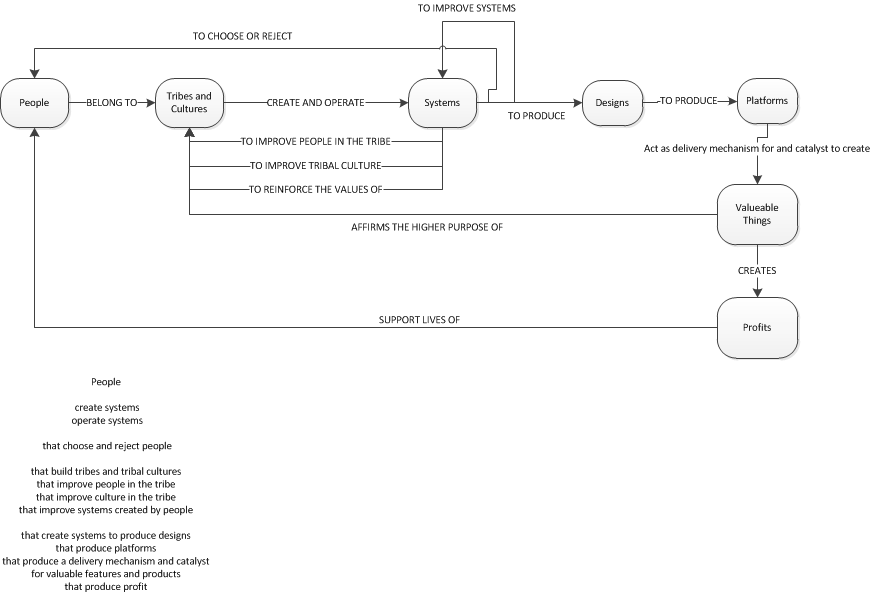
\includegraphics[width=\textwidth]{SystemCreation.png}
\caption{The positive feeback cycle between tribes, people, systems and company profit. \textcopyright Grant Reid}
\label{fig:peoplesystems}
\end{figure*}

\section{The Key Problems}
Three key problems are inhibiting growth. They are purpose switching, fear of
failure, and singular points of view. Each one of these problems inhibit
the positive feedback cycle shown in figure \ref{fig:peoplesystems}.

\subsection{Purpose Switching}
ORGX has multiple purposes. Different parts of the organisation deal with one
or maybe more of those purposes. Purpose switching often is mistaken for
task switching. Task switching is hard, but is usually within the same buiness
context. Purpose switching changes business context as well as the task. Parts
of ORGX are constantly switching context. Because context switching is difficult
people generally stay within a single context. This leads to singluar points of
view (\ref{sec:singularPointOfView}) which increases confusion. Confusion in
combination with pressure to achieve results in the inability to think
objectively. This inability to think objectively cripples parts of ORGX and is
a negative cycle. 

\subsection{Fear of Fail}
When did I do my most learning. University. Why? I failed heaps.



\subsection{Singular Point of View}
\label{sec:singularPointOfView}
Three objects are sitting on a table. A rugby ball, tennis ball and a \emph{gold
golf ball}. An objective is set for two people. They are asked to take the
object of most value. They both sit down on next to each other and look at the objects
from different perspectives. One can see the golf ball, the other can not. How
does the person who sees the golf ball convince the other that it is there?

The above situation is a simplifcation of what happens when multiple people are
ask to solve a problem. Depending on the dynamics of the group, results
will vary. At ORGX there is an inablity to belief there is a \emph{gold golf
ball}. This usually leads to fighting because there is an absense of trust.
Furthermore, individuals prefer to stay fixed in the company purpose (or
viewpoint) because it is comfortable. Fear of leaving this confort zone is
preceived a too higher risk. Just like most electrons most humans love to find
their lowest possible energy state.

\section{Designing the Light Bulb}
Essentially people need to feel that they create and operate systems that
produce valuable things. This affirms their purpose and empowers them.

The first step will be called Freedom Fridays.

\subsection{Freedom Fridays}
Freedom fridays provides the opportunity for staff to think with a fresh mind
one day a week. 


\subsubsection{Risks}
\begin{itemize}
    \item People spending more than there alloted amount. (This should be
mitigated by people behaving as professions. I.E. when work needs to be done they may use
their freedom time to do it.)
    \item Middle managers place control over what people work on. (Mitigated by
leadership training PDLC - You have your people for 80 percent of time. Make
their time valuble)
    \item People go cowboy with idea (start selling etc..) Mitigated by new technology
manager/team. 
    \item An Empty second step. Providing freedom friday without the supporting
mechanisms will add to the confusion. The message needs to be clear and
followed by actions.
\end{itemize}

\subsection{Next Steps}
\begin{itemize}
    \item Present a problem, present a solution - Any team
    \item Emotional Intelligence course. Increase EQ. People need to be aware of their
amgdala hyjacks
    \item Paradigm breaking - S-Curve, you don't have to build it to sell the
    idea.
    \item Innovation pipeline. Need to come up with method so employees can turn their
free ideas (if they want to) into company products.
\end{itemize}

\section{Conclusion}
The conclusion goes here.

\end{document}

